\section{Introduction aux composants natifs}
\subsection{Les composants natifs}
Les composants natifs sont des composants mis à disposition par {\color{monOrange}Vue} pour certains effets avancés comme par exemple la mise en cache, les transitions etc. Dans ce chapitre nous allons voir les composants natifs suivants :
\begin{itemize}
\item {\tt <Component>:} qui permet de créer des composants dynamiques.
\item {\tt <KeepAlive>:} qui permet une mise en cache des composants.
\item {\tt <Teleport>:} qui permet de "téléporter" une partie d'un {\color{monOrange}template} d'un composant à l'extérieur de l'application {\color{monOrange}Vue}.
\item {\tt <Suspense>:} qui permet de gérer les dépendances asynchrones d'un arbre de composant.
\end{itemize}
\subsection{Les composants dynamiques}
Il est parfois utile de pouvoir changer dynamiquement de composant. Par exemple pour une interface avec des onglets. Avec le composant natif {\color{monOrange}Component}, et l'attribut {\color{monOrange}is} à lié une variable contenant le nom d'un composant, il est facile de mettre en place une telle interface :
\begin{minted}[
mathescape,
framesep=2mm,
baselinestretch=1.2,
fontsize=\footnotesize,
bgcolor=LightGray,
%linenos
]{html}
<Component :is="onglet" />
\end{minted}
Cette fonctionnalité est assez rarement utilisée avec le {\color{monOrange}Router} que nous verrons plus tard, nous ne détaillerons donc pas plus.
\subsection{Exemple}
\begin{minted}[
mathescape,
framesep=2mm,
baselinestretch=1.2,
fontsize=\footnotesize,
bgcolor=LightGray,
%linenos
]{html}
<template>
  <div class="p-20">
    <button @click="selectedComponant = 'PageA'" class="btn btn-danger mr-10">
      Page A
    </button>
    <button @click="selectedComponant = 'PageB'" class="btn btn-primary mr-10">
      Page B
    </button>
    <Component :is="composants[selectedComponant]" />
  </div>
</template>

<script setup lang="ts">
import PageA from './PageA.vue';
import PageB from './PageB.vue';
import { ref, type Component as C } from 'vue';

const composants: { [s:string]: C } = {
  PageA,
  PageB,
};

const selectedComponant = ref('PageA');
</script>

<style lang="scss">
@import './assets/scss/base.scss';
</style>
\end{minted}
\begin{center}
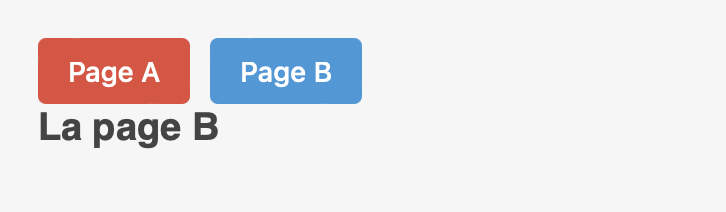
\includegraphics[width=7cm]{images/image29.png}
\end{center}
%%%%%%%%%%%%%%%%%%%%%%%%%%%%%%%%%%%%%%%%%%%%%%%%%%%

\section{Le composant KeepAlive}
\subsection{Le composant {\color{monOrange}KeepAlive}}
Le composant natif {\tt <KeepAlive>} permet de mettre en cache conditionnellement des composants lorsque l'on change dynamiquement de composant . En effet, par défaut une instance d'un composant {\color{monOrange}Vue} est démontée ( {\color{monOrange}unmounted}) lorsqu'il n'est plus affiché. Cela entraîne la perte de tout état du composant. Autrement dit, lorsqu'un composant n'est plus affiché, toutes les variables, notamment réactives, perdent leurs valeurs.

Lorsqu'un composant mis en cache avec {\tt <KeepAlive>} est retiré du {\color{monOrange}DOM}, il est mis dans l'état désactivé ({\tt deactivated}) au lieu d'être démonté ( {\tt unmounted}).

Lorsque le composant est remis sur le {\color{monOrange}DOM} aura alors l'état est activé ( {\tt activated}). Il suffit d'imbriquer, le ou les composants à l'intérieur du composant {\tt <KeepAlive>}, par exemple :
\begin{minted}[
mathescape,
framesep=2mm,
baselinestretch=1.2,
%fontsize=\footnotesize,
bgcolor=LightGray,
%linenos
]{html}
<KeepAlive>
  <Component :is="onglet" />
</KeepAlive>
\end{minted}

\subsection{Définir les composants à maintenir en vie avec {\color{monOrange}includes} et {\color{monOrange}exclude}}
Par défaut, {\tt <KeepAlive>} mis en cache tous les composants imbriqués. Il est possible de modifier ce comportement avec les {\color{monOrange}props include} et {\color{monOrange}exclude}. Pour utiliser cette fonctionnalité, il faut préalablement que les composants soient nommés en utilisant une deuxième balise {\color{monOrange}script} et en utilisant la propriété {\tt name}, comme ici :
\begin{minted}[
mathescape,
framesep=2mm,
baselinestretch=1.2,
%fontsize=\footnotesize,
bgcolor=LightGray,
%linenos
]{html}
<script lang="ts">
export default {
  name: 'PageB',
};
</script>
\end{minted}
Il suffit ensuite de préciser les composants à mettre en cache en utilisant {\color{monOrange}include} ou {\color{monOrange}exclude}:
\begin{minted}[
mathescape,
framesep=2mm,
baselinestretch=1.2,
%fontsize=\footnotesize,
bgcolor=LightGray,
%linenos
]{html}
<KeepAlive include="PageB">
  <Component :is="composants[selectedComponant]" />
</KeepAlive>
\end{minted}
Vous pouvez utiliser des {\color{monOrange}Regex}:
\begin{minted}[
mathescape,
framesep=2mm,
baselinestretch=1.2,
%fontsize=\footnotesize,
bgcolor=LightGray,
%linenos
]{html}
<KeepAlive include="/Page*/">
  <Component :is="composants[selectedComponant]" />
</KeepAlive>
\end{minted}
Passer plusieurs noms en utilisant des virgules :
\begin{minted}[
mathescape,
framesep=2mm,
baselinestretch=1.2,
%fontsize=\footnotesize,
bgcolor=LightGray,
%linenos
]{html}
<KeepAlive exclude="PageA, PageC">
  <Component :is="composants[selectedComponant]" />
</KeepAlive>
\end{minted}
Ou un tableau :
\begin{minted}[
mathescape,
framesep=2mm,
baselinestretch=1.2,
%fontsize=\footnotesize,
bgcolor=LightGray,
%linenos
]{html}
<KeepAlive exclude="['PageA', 'PageC']">
  <Component :is="composants[selectedComponant]" />
</KeepAlive>
\end{minted}
\subsection{Définir le maximum de composants mis en cache}
Si vous avez un très grand nombre de composants susceptibles d'être mis en cache, vous pouvez limiter le nombre maximal de composants à mettre en cache avec la {\color{monOrange}props max}. Il faut utiliser {\color{monOrange}v-bind} car nous passons un nombre (comme nous l'avions vu, sans {\color{monOrange}v-bind} les nombres sont passés comme des chaînes de caractères) :
\begin{minted}[
mathescape,
framesep=2mm,
baselinestretch=1.2,
%fontsize=\footnotesize,
bgcolor=LightGray,
%linenos
]{html}
<KeepAlive :max="10">
  <Component :is="activeComponent" />
</KeepAlive>
\end{minted}
\subsection{Les {\color{monOrange}hooks} utilisables}
Il est possible d'utiliser les {\tt hooks:} {\color{monOrange}activated()} et {\color{monOrange}deactivated()}.
\begin{minted}[
mathescape,
framesep=2mm,
baselinestretch=1.2,
%fontsize=\footnotesize,
bgcolor=LightGray,
%linenos
]{html}
<script setup lang="ts">
import { onActivated, onDeactivated } from 'vue'

onActivated(() => {
  // appelé à chaque activation du composant
})

onDeactivated(() => {
  // appelé à chaque désactivation du composant
})
</script>
\end{minted}

\subsection{Exemple}
On reprend l'exemple précédant et on modifie {\tt App.vue} de la façon suivante:
\begin{minted}[
mathescape,
framesep=2mm,
baselinestretch=1.2,
fontsize=\footnotesize,
bgcolor=LightGray,
%linenos
]{html}
<KeepAlive :max="5">
      <Component :is="composants[selectedComponant]" />
</KeepAlive>
\end{minted}
On modéfie {\tt PageA.vue} et {\tt PageB.vue}:
\begin{minted}[
mathescape,
framesep=2mm,
baselinestretch=1.2,
%fontsize=\footnotesize,
bgcolor=LightGray,
%linenos
]{html}
<template>
  <h3>La page A</h3>
  <br />
  <button class="btn mb-20" @click="count++">{{ count }}</button>
</template>

<script setup lang="ts">
import { ref, onDeactivated } from 'vue';

const count = ref(0);

onDeactivated(() => {
  count.value--;
});
</script>

<style scoped lang="scss"></style>
\end{minted}
puis on fait
\begin{minted}[
mathescape,
framesep=2mm,
baselinestretch=1.2,
fontsize=\footnotesize,
bgcolor=LightGray,
%linenos
]{html}
<template>
  <h3>La page B</h3>
  <br />
  <span>Utilisateur : {{ username }}</span>
  <input v-model="username" />
</template>

<script lang="ts">
export default {
  name: 'PageB',
};
</script>

<script setup lang="ts">
import { ref, onActivated } from 'vue';
const username = ref('');

onActivated(() => {
  username.value += '!';
});
</script>

<style scoped lang="scss"></style>
\end{minted}
On teste le resultat:
\begin{center}
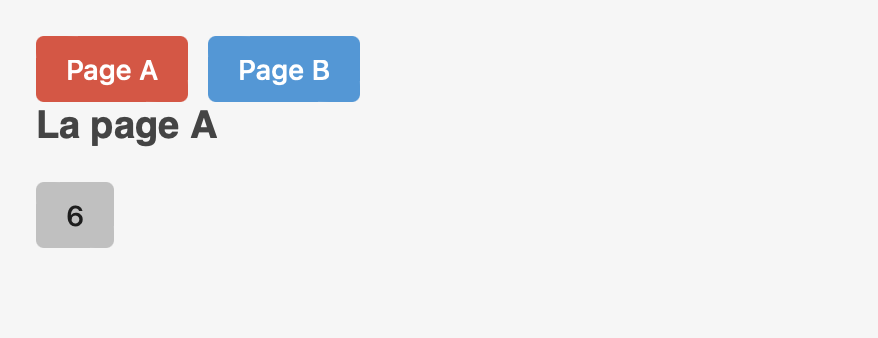
\includegraphics[width=7cm]{images/image30.png}
\end{center}


%%%%%%%%%%%%%%%%%%%%%%%%%%%%%%%%%%%%%%%%%%%%%%%%%%%%%%%%%%%%%

\section{Le composant Téléport}
\subsection{Le composant natif {\color{monOrange}Teleport}}
{\tt <Teleport>} est un composant natif permettant de {\em téléporter} une partie du {\color{monOrange}template} un composant sur un noeud du {\color{monOrange}DOM} qui existe en dehors de la branche du composant, ou même en dehors de l'application {\color{monOrange}Vue}.

Le scénario le plus commun est la modale : une partie d'un composant doit être affichée ailleurs sur le {\color{monOrange}DOM}, à l'extérieur de l'application. Nous voulons en effet que le bouton de la modale et la modale soient dans le même composant, car ils sont tous deux liés à l'état ouvert/fermé de la modale. Mais cela signifie que le modal sera rendu à côté du bouton, profondément imbriquée dans l'arbre des composants de l'application {\color{monOrange}Vue}. Cela peut créer des problèmes lors du positionnement de la modale avec du {\color{monOrange}CSS}. L'utilisation est très simple, il suffit d'imbriquer la partie du {\color{monOrange}template} "téléporter" dans des balises {\tt <Teleport>} et d'indiquer avec le {\color{monOrange}props to} sélecteur {\color{monOrange}CSS} ciblé :
\begin{minted}[
mathescape,
framesep=2mm,
baselinestretch=1.2,
%fontsize=\footnotesize,
bgcolor=LightGray,
%linenos
]{html}
<button @click="open = true">Ouvrir</button>

<Teleport to="body">
  <div v-if="open" class="modal">
    <p>Contenu de la modale</p>
    <button @click="open = false">Fermer</button>
  </div>
</Teleport>
\end{minted}
Il est possible de désactiver la téléportation du {\color{monOrange}template} en fonction de la valeur d'une variable en utilisant {\color{monOrange}disabled}:
\begin{minted}[
mathescape,
framesep=2mm,
baselinestretch=1.2,
fontsize=\footnotesize,
bgcolor=LightGray,
%linenos
]{html}
<Teleport :disabled="isMobile">
  ...
</Teleport>
\end{minted}
\subsection{Exemple}
\subsubsection*{App.vue}
\begin{minted}[
mathescape,
framesep=2mm,
baselinestretch=1.2,
%fontsize=\footnotesize,
bgcolor=LightGray,
%linenos
]{html}
<template>
  <Page />
</template>

<script setup lang="ts">
import Page from './Page.vue';
</script>

<style lang="scss">
@import './assets/scss/base.scss';
</style>
\end{minted}
\subsubsection*{Page.vue}
\begin{minted}[
mathescape,
framesep=2mm,
baselinestretch=1.2,
fontsize=\footnotesize,
bgcolor=LightGray,
%linenos
]{html}
<template>
  <div class="p-20 container">
    <h3>PAGE</h3>
    <Modal />
  </div>
</template>

<script setup lang="ts">
import Modal from './Modal.vue';
</script>

<style lang="scss">
.container {
  position: relative;
}
</style>
\end{minted}
\subsubsection*{Modal.vue}
\begin{minted}[
mathescape,
framesep=2mm,
baselinestretch=1.2,
fontsize=\footnotesize,
bgcolor=LightGray,
%linenos
]{html}
<template>
  <button @click="open = true" class="btn btn-primary">
    Confirmer l'achat
  </button>
  <Teleport to="body">
    <div
      v-if="open"
      @click="open = false"
      class="calc d-flex flex-row justify-content-center align-items-center"
    >
      <div @click.stop class="modal-container">
        <h3>Confirmation de votre commande</h3>
        <ul>
          <li>Du contenu</li>
          <li>Du contenu</li>
          <li>Du contenu</li>
        </ul>
        <button @click.stop="open = false" class="btn btn-danger">
          Confirmer la commande
        </button>
      </div>
    </div>
  </Teleport>
</template>

<script setup lang="ts">
import { ref } from 'vue';

const open = ref(false);
</script>

<style lang="scss">
.calc {
  position: absolute;
  top: 0;
  width: 100%;
  height: 100vh;
  background-color: rgba(0, 0, 0, 0.5);
  backdrop-filter: blur(2px);
}

.modal-container {
  background-color: white;
  border-radius: var(--border-radius);
  border: var(--border);
  padding: 30px;
}
</style>
\end{minted}
\begin{center}
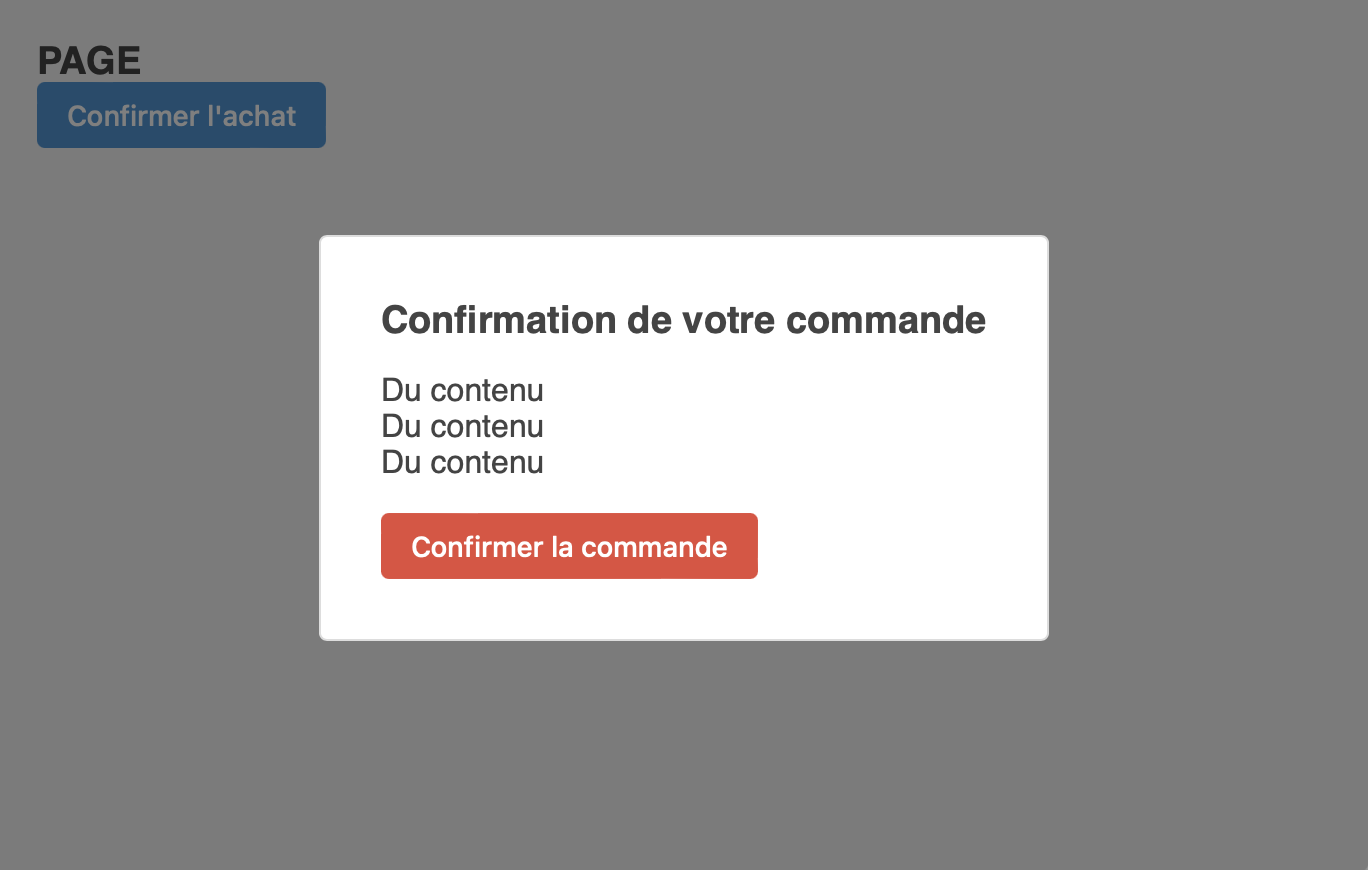
\includegraphics[width=10cm]{images/image31.png}
\end{center}
%%%%%%%%%%%%%%%%%%%%%%%%%%%%%%%%%%%%%%%%%%%%%%%%%%%%%%%%%%%%%%

\section{Le composant Suspense}
\subsection{Le composant {\tt <Suspense>}}
{\tt <Suspense>} est un composant natif permettant de gérer les dépendances asynchrones d'une branche de composants . Il permet d'afficher un {\color{monOrange}template} spécifique pendant le chargement des différentes ressources asynchrones. Les ressources asynchrones sont la plupart du temps des requêtes {\color{monOrange}HTTP} pour récupérer des données depuis une {\color{monOrange}API}. Il peut y avoir un composant qui a besoin d'une liste d'utilisateurs, un autre qui a besoin de favoris, un troisième de préférences utilisateur avec des requêtes différentes.

Sans {\color{monOrange}Suspense} il faut que chaque composant gère l'affichage d'un composant de chargement, des éventuelles erreurs etc. Cela permet de simplifier grandement la gestion des ressources asynchrones.

Le composant {\color{monOrange}Suspense} peut gérer deux types de dépendances asynchrones : les composants qui utilisent des {\color{monOrange}await} au premier niveau (c'est-à-dire pas imbriqué dans une fonction, directement dans les balises {\color{monOrange}script}) et les composants asynchrones .

Pour les composants avec {\color{monOrange}await} au premier niveau, le cas le plus courant est une requête {\color{monOrange}HTTP}:
\begin{minted}[
mathescape,
framesep=2mm,
baselinestretch=1.2,
%fontsize=\footnotesize,
bgcolor=LightGray,
%linenos
]{html}
<script setup>
const res = await fetch(...)
const posts = await res.json()
</script>
\end{minted}
\subsection{État de chargement}
Le composant {\color{monOrange}Suspense} à deux {\color{monOrange}slots} nommés : {\color{monOrange}\#default} et {\color{monOrange}\#fallback} . Chaque {\color{monOrange}slot} permet l'utilisation d'un unique enfant : que ce soit un composant ou un élément {\color{monOrange}HTML}:
\begin{minted}[
mathescape,
framesep=2mm,
baselinestretch=1.2,
%fontsize=\footnotesize,
bgcolor=LightGray,
%linenos
]{html}
<Suspense>
  <Dashboard />
  <template #fallback>
    Chargement...
  </template>
</Suspense>
\end{minted}
Lors du rendu initial, {\color{monOrange}Suspense} va afficher le {\color{monOrange}slot} par défaut (ici le composant {\color{monOrange}Dashbord}, car le {\color{monOrange}slot default} est l'élément qui n'a pas de nom). S'il rencontre une dépendance asynchrone, {\color{monOrange}Suspense} va entrer dans l'état en attente ( {\color{monOrange}pending state}). Pendant toute la durée de cet état, il affichera le {\color{monOrange}slot fallback}, ici {\tt <template \#fallback>}.

Lorsque tous les contenus asynchrones sont chargés ou qu'il n'y a aucune dépendance asynchrone, alors {\color{monOrange} Suspense} à l'état résolu ( {\color{monOrange}resolved state}) et le {\color{monOrange}slot} par défaut est affiché.

\subsection{Les événements émis}
Le composant {\color{monOrange}Suspense} émet trois événements :
\begin{itemize}
\item {\color{monOrange}pending:} émis lorsqu'il entre dans l'état pendinget donc qu'au moins une dépendance asynchrone a été détectée.
\item {\color{monOrange}resolve:} émis lorsqu'aucune dépendance asynchrone ne reste à charger.
\item {\color{monOrange}fallback:} émis lorsque le composant Suspense affiche le {\color{monOrange}slot fallbacklors} du chargement des dépendances asynchrones.

\end{itemize}
\subsection{Option {\color{monOrange}timeout}}
Lorsque le composant {\color{monOrange}Suspense} est dans l'état résolu, il ne retournera dans l'état en attente que si un composant dynamique est modifié et que la propriété {\color{monOrange}timeout} est définie. En effet, par défaut, {\color{monOrange}Suspense} affichera le composant par défaut et non le {\color{monOrange}fallback} pendant le chargement des dépendances asynchrones dans ce cas.

Il est possible de passer un nombre de millisecondes à {\color{monOrange}timeout} pour que {\color{monOrange}Suspense} affiche le {\color{monOrange}fallback} pendant le chargement, si les dépendances ne sont pas résolues pendant ce laps de temps.
\subsection{Exemple}
\subsubsection*{App.vue}
\begin{minted}[
mathescape,
framesep=2mm,
baselinestretch=1.2,
fontsize=\footnotesize,
bgcolor=LightGray,
%linenos
]{html}
<template>
  <h2>{{ evenement }}</h2>
  <Suspense
    @pending="myEvent('PENDING')"
    @fallback="myEvent('FALLBACK')"
    @resolve="myEvent('RESOLVE')"
  >
    <LazyList />
    <template #fallback>
      <h1>Chargement...</h1>
    </template>
  </Suspense>
</template>

<script setup lang="ts">
import { defineAsyncComponent, ref } from 'vue';

const evenement = ref('');
const LazyList = defineAsyncComponent(() => import('./Liste.vue'));

function myEvent(eventName: string) {
  console.log(eventName);
  evenement.value = eventName;
}
</script>

<style lang="scss"></style>
\end{minted}
\subsubsection*{Liste.vue}
\begin{minted}[
mathescape,
framesep=2mm,
baselinestretch=1.2,
fontsize=\footnotesize,
bgcolor=LightGray,
%linenos
]{html}
<template>
  <div class="p-20">
    <ul>
      <li v-for="user of state.users">{{ user.name }}</li>
    </ul>
  </div>
</template>

<script setup lang="ts">
import { reactive } from 'vue';

const state = reactive<{ users: any[] }>({ users: [] });

// Délai de 3secondes grâce à l'option delay de restapi
state.users = await (
  await fetch('https://restapi.fr/api/vueusers?delay=3')
).json();
</script>

<style lang="scss"></style>
\end{minted}
\begin{center}
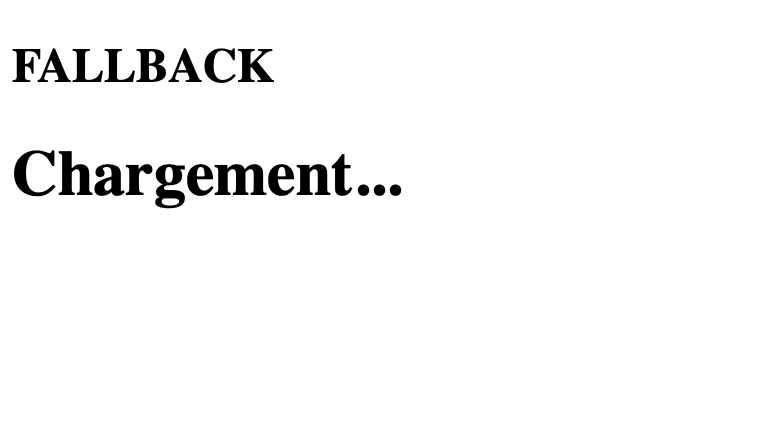
\includegraphics[width=7cm]{images/image32.png}
\end{center}
